\title{Dither watermarking round trip}

 \begin{verbatim}
 Il me semble  qu'il  faudrait  faire  le  simulateur complet. Une fois qu'il
 est fait, on l'aurait une fois pour toutes et  on  pourrait l'utiliser pour
 d'autres projets SURYS.

 Input : une image
 -générer un message texte aléatoire  de la  longueur prescrite
 -le coder avec une redondance  suffisante (récupérer un code de codage
 vectoriel standard?)
 -l'insérer dans  le dithering de l'image
 -dans l'ordre:  lui ajouter quelques  anomalies destructives (Axel et
 Thibaud ont  un simulateur d'anomalies locales style  rayures),  la
 déformer, la rendre floue et  la  bruiter
 -détecter la  grille et  décoder
 On  peut  en discuter quand vous  voulez; le sujet me paraît très
 intéressant,  en fait  pour nous  entraîner  à la  stéganographie.
 Amitiés,
 JM
 \end{verbatim}


\section{Encoding data into binary image}

For our encoding/decoding experiments we work with the full text of
Shakespeare sonnets.  We use it as a periodic, infinite stream of bits, of
period 96Kb or 771024 bits (starting at sonnet CXXX, one of the most famous).
Notice that the ASCII encoding of text is very inefficient; in practice we
would use a compressed stream;  this is just for verification.

The carrier image is a black and white photo, that we reduce to a small size
and binarize by a linear retinex filter and Floyd-Sternberg dithering:

\begin{tabular}{cccc}
	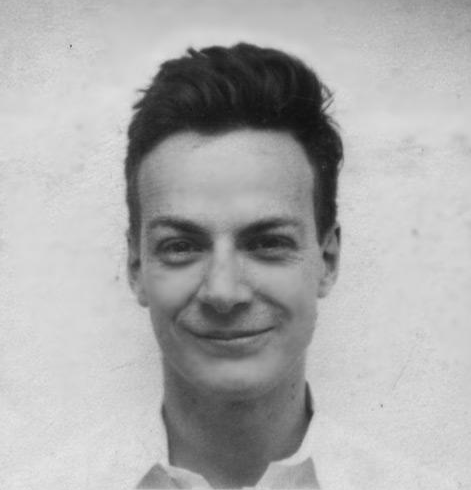
\includegraphics{i/feynman.png} &
	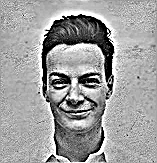
\includegraphics{a0.png} &
	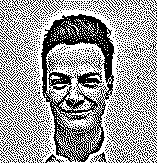
\includegraphics{a.png} &
	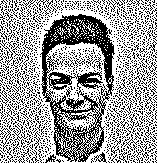
\includegraphics{a-sonnet.png} \\
	\verb+feynman.png+ &
	\verb+a0.png+ &
	\verb+a.png+ &
	\verb+a-sonnet.png+
\end{tabular}

%RUN_VERBATIMS sh
\begin{verbatim}
ppsmooth i/feynman.png|downsa v 3|plambda 'x,l -1 *'|blur q 0.2|qauto - a0.png
dither a0.png a.png
mdither encode a.png a-sonnet.png < i/sonnets.txt
\end{verbatim}

This image has enough space to encode one sonnet and the title of
the next one.  It can be
recovered with the program \verb+mdither decode+:

 \begin{verbatim}
mdither decode a-sonnet.png
\end{verbatim} %

 \begin{verbatim}
 Sonnet CXXX

 My mistress' eyes are nothing like the sun;
 Coral is far more red than her lips' red;
 If snow be white, why then her breasts are dun;
 If hairs be wires, black wires grow on her head.
 I have seen roses damask'd, red and white,
 But no such roses see I in her cheeks;
 And in some perfumes is there more delight
 Than in the breath that from my mistress reeks.
 I love to hear her speak, yet well I know
 That music hath a far more pleasing sound;
 I grant I never saw a goddess go;
 My mistress, when she walks, treads on the ground:
 And yet, by heaven, I think my love as rare
 As any she belied with false compare.

 Sonnet CXXXI

\end{verbatim} %


\section{Printing and acquisition}

Now that we can encode and decode data into binary images, we will see if
this data is recoverable after printing the image into paper and scanning
it/taking a photo.  For that, we propose the following algorithm that tries
to simulates a realistic acquisition process with various distortions.

\subsection{Zoom-in the image and reduce its contrast}

\begin{verbatim}
export GETPIXEL=255
ntiply 4 a-sonnet.png|plambda zero:800x800 - "x y(-90,-70) -50 320 qe" -o a2.png
plambda a2.png randu | blur l 170 | qauto - biases.png
plambda a2.png biases.png "x .6 * y .4 * +" -o a3.png
\end{verbatim}
\begin{gallery}
	\galleryline{a3.png}
	\galleryline{a2.png}
	\galleryline{biases.png}
\end{gallery}
%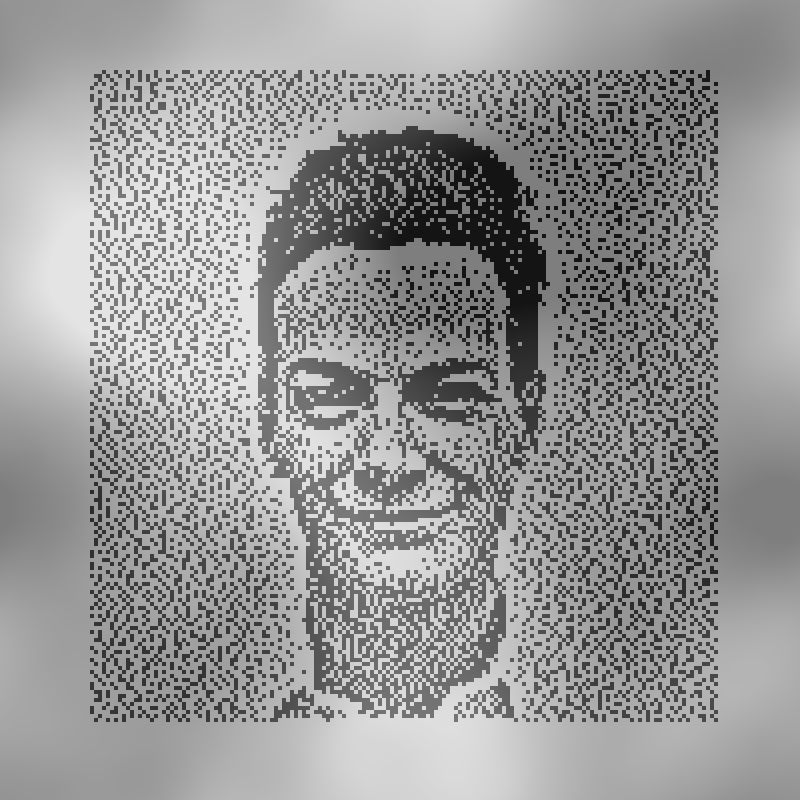
\includegraphics{a3.png}\verb+a3.png+

\subsection{Apply an homography}
\begin{verbatim}
H="1 0 100  0 1 100  0.0002 -0.0001 1"
homwarp -o 3 -i "$H" 1000 1000 a3.png a4.png
\end{verbatim}
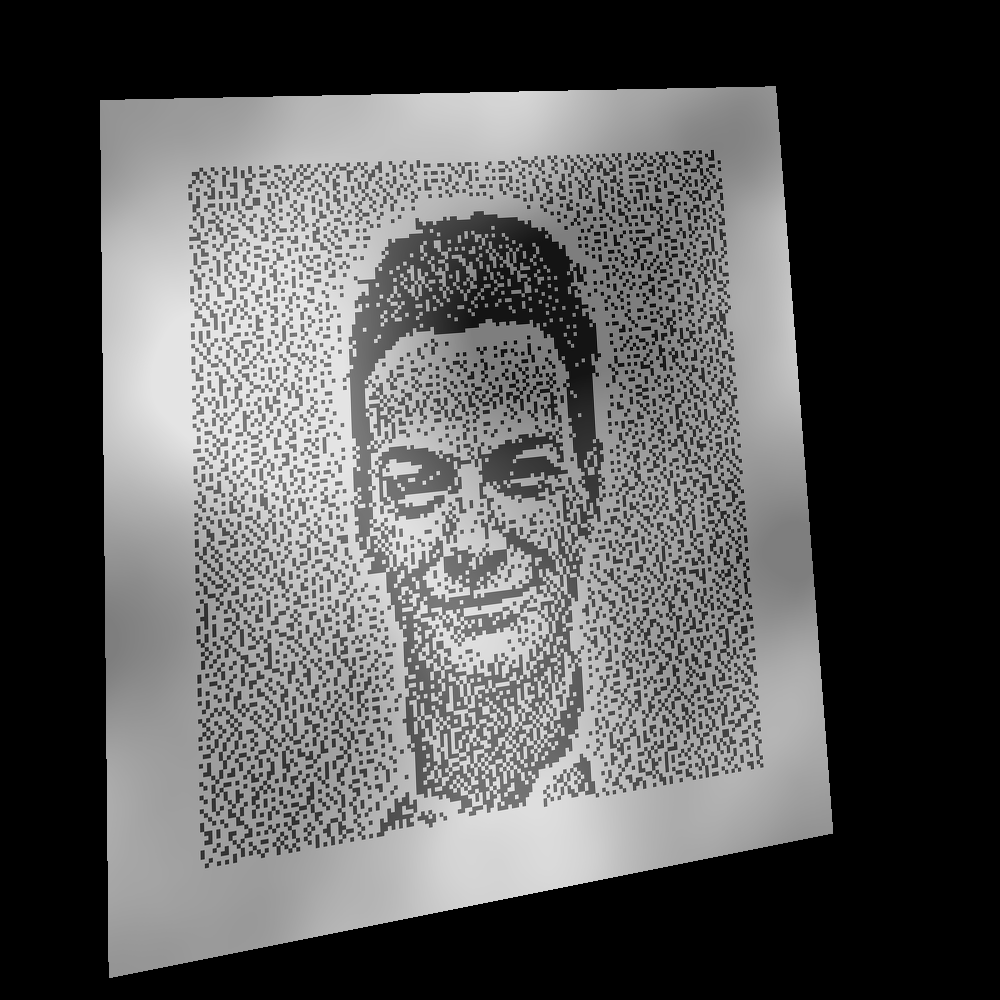
\includegraphics{a4.png}\verb+a4.png+

\subsection{Apply a small non-rigid deformation}
\begin{verbatim}
sepranfield.sh 1000 1000 2 g 200 g 14 1 | backflow - a4.png a5.png
\end{verbatim}
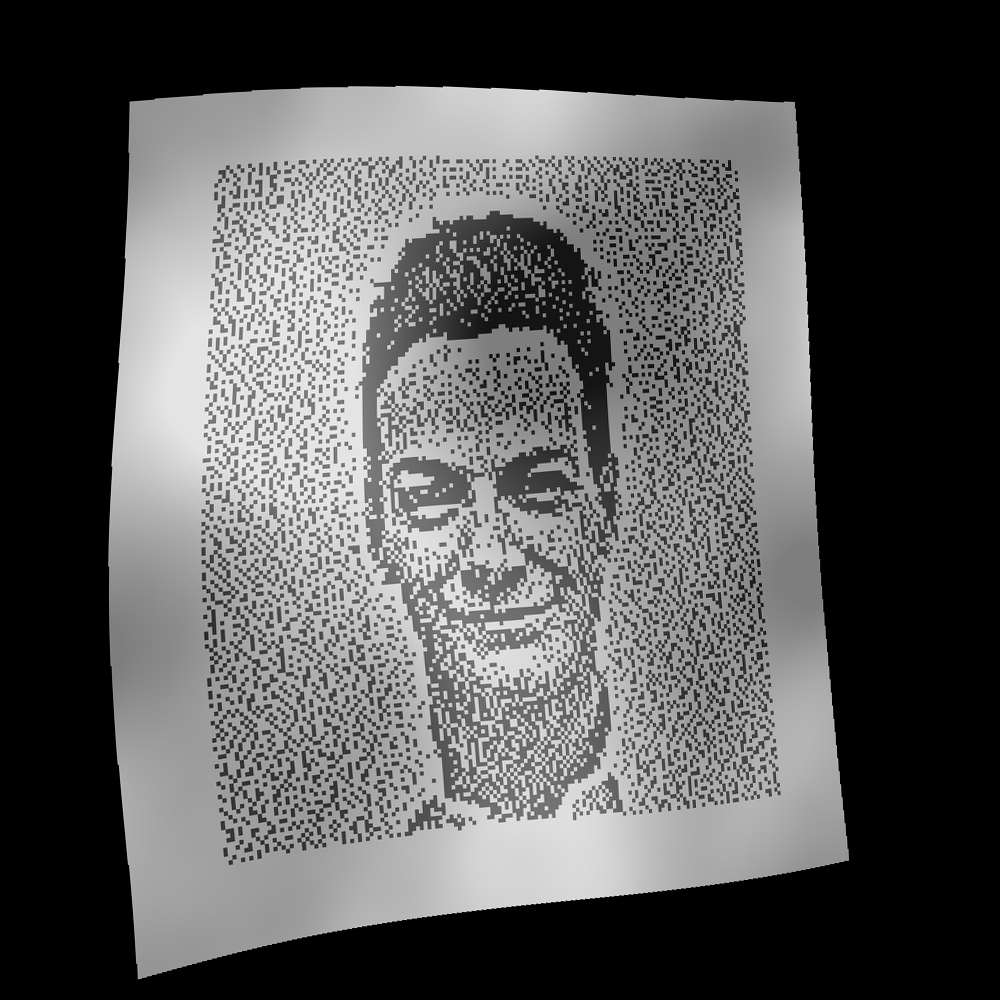
\includegraphics{a5.png}\verb+a5.png+

\subsection{Add a textured background}
\begin{verbatim}
plambda a5.png randg | blur q 0.5 | qauto -p 0 - bg.png
plambda a5.png "0 >" | morsi cross closing - mask.png
plambda mask.png a5.png bg.png if -o a6.png
\end{verbatim}
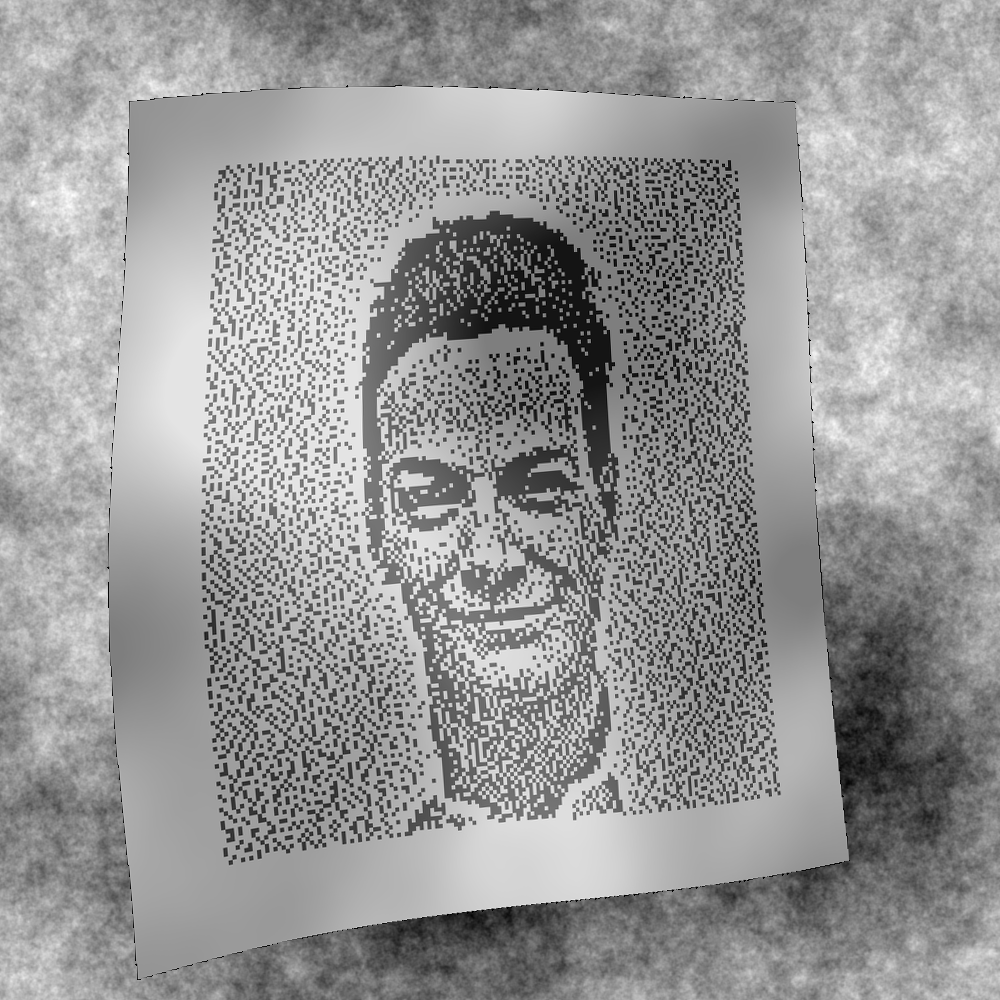
\includegraphics{a6.png}\verb+a6.png+

\subsection{Add blur and noise}
\begin{verbatim}
blur gauss 1.5 a6.png | plambda - "randg 5 * +" -o dirty.png
\end{verbatim}
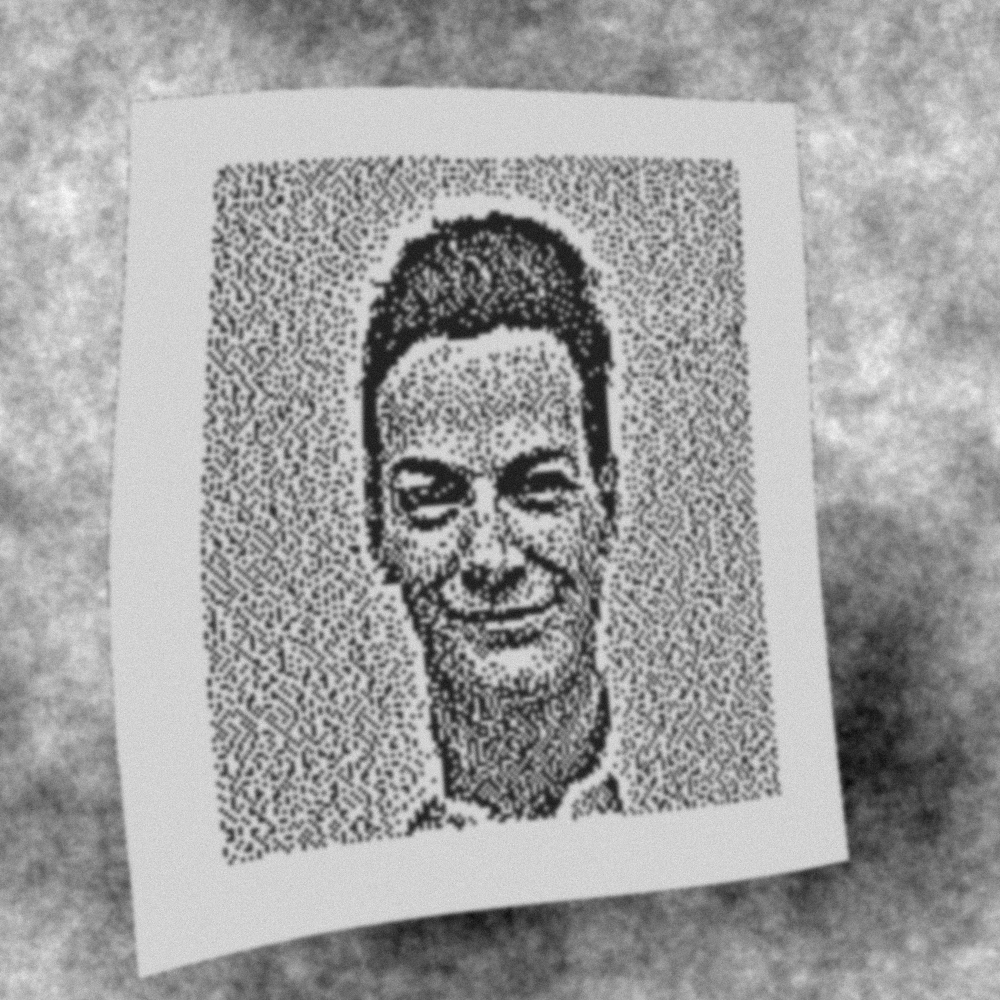
\includegraphics{dirty.png}\verb+dirty.png+

\subsection{Optionally: add some holes}
\begin{verbatim}
plambda bg.png 'randp 1.2 ^'                    |\
        blur q 0.25                             |\
        plambda - mask.png "y x x%O92 < and"    |\
        plambda - a6.png bg.png if            |\
        blur g 1.5                              |\
        plambda - "randg 5 * +" -o dirtier.png
\end{verbatim}
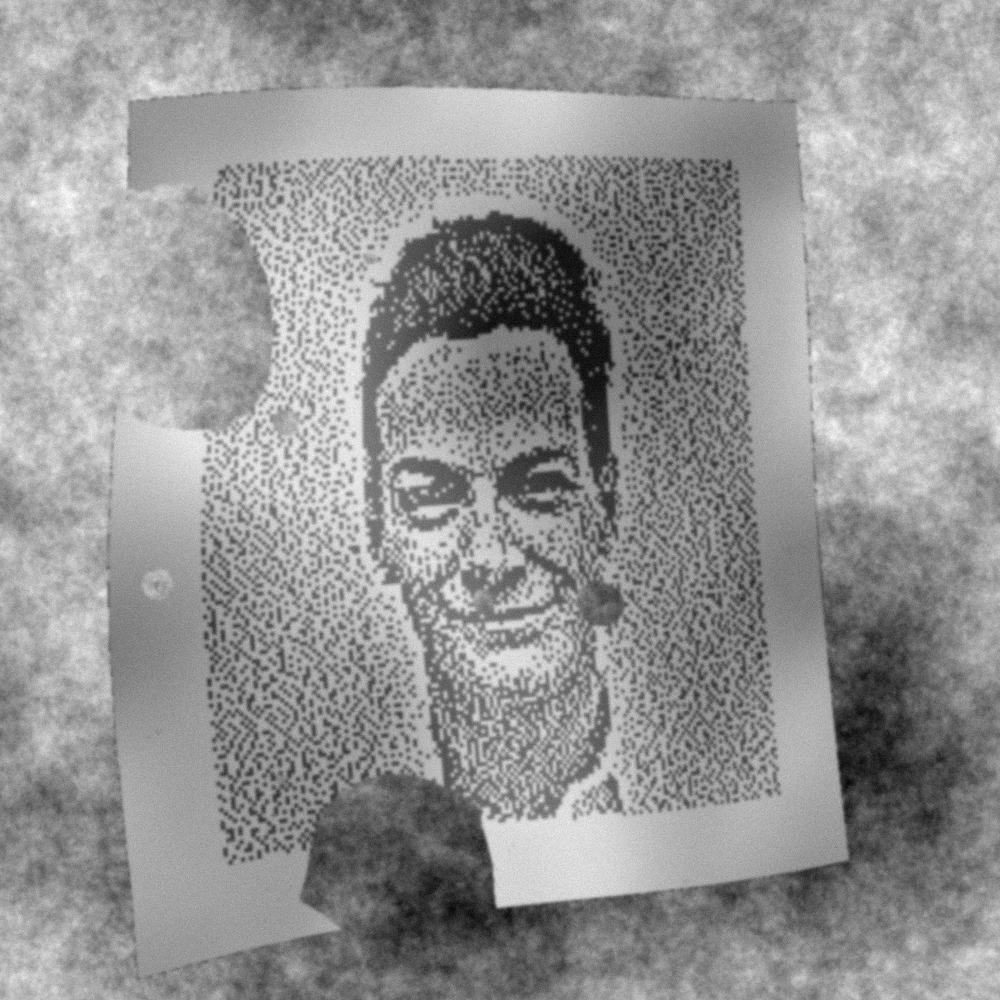
\includegraphics{dirtier.png}\verb+dirtier.png+

\section{Recovery of the dithered image}

Recovery of the image data consists in inverting all the steps of the
simulation algorithm.  This is easier said than done.  To simplify the
problem, we start with the easy case of no deformation (so that an homography
is able to recover the exact position of the grid) and no holes (so that
there is no missing data).

In this ideal case, we need to start with this image (without deformation nor
holes):
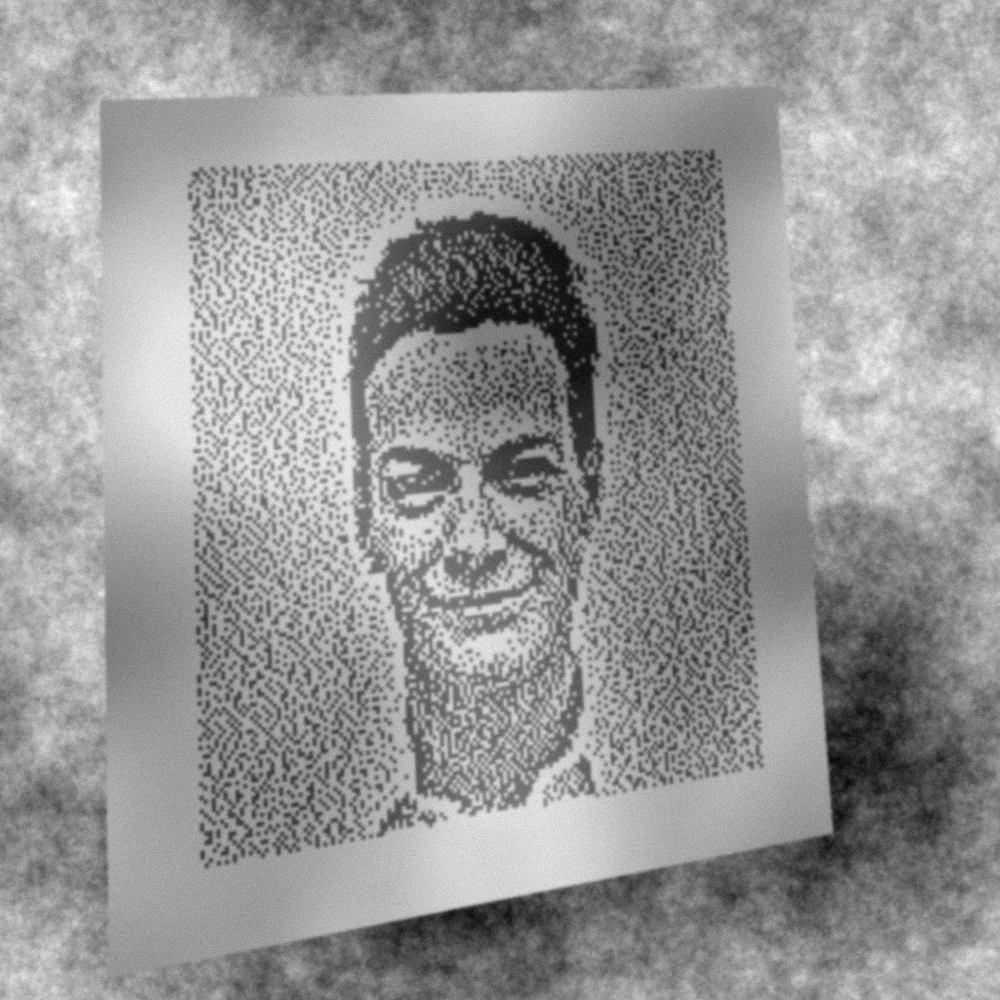
\includegraphics{easy.png}\verb+easy.png+
\begin{verbatim}
plambda a4.png "0 >"                           |\
        morsi cross closing                    |\
        plambda - a4.png bg.png if             |\
        blur gauss 1.5                         |\
        plambda - "randg 5 * +" -o easy.png
\end{verbatim}

which, given the correct  homography, can only be recovered as good as this:
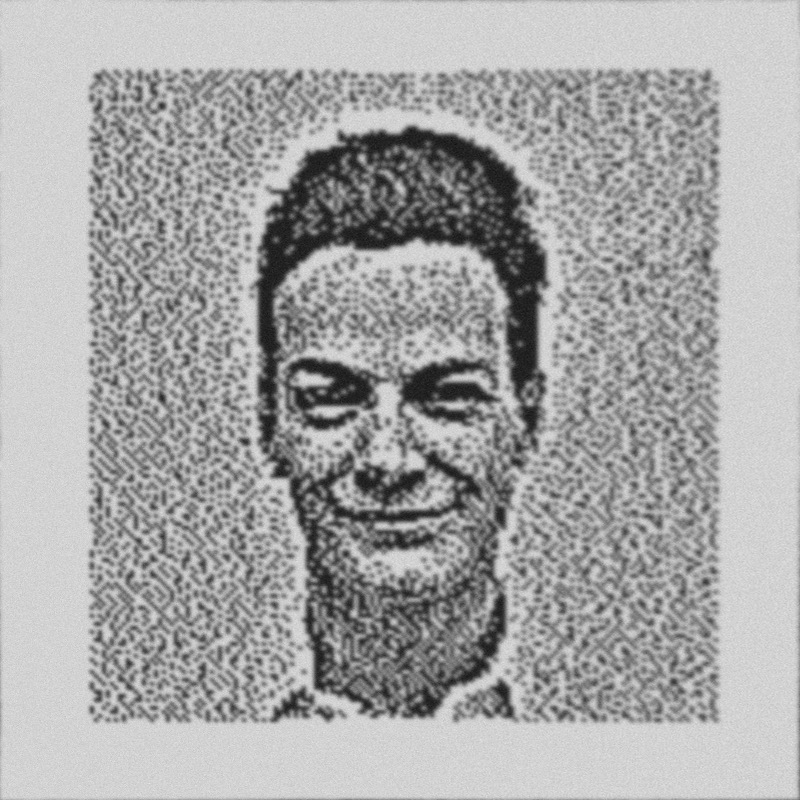
\includegraphics{recov.png}\verb+recov.png+
\begin{verbatim}
homwarp -o 3 "$H" 800 800 easy.png recov.png
\end{verbatim}
can you find a grid of size 157x163 in here?  Since we now the exact sizes,
let us see how well can we recover the bits in this case (a retinex of the
zoomed-image helps to discriminate binary pixels):


%cat clip.png | downsa v 4 | ntiply 4 | qauto -p 0 - rec2.png
%plambda rec2.png 'x,l -1 *'|blur -z z 0.3|plambda - '0 > 255 *' -o ret-rec2.png

\begin{verbatim}
plambda zero:628x652 recov.png "x y(90,70)" -o clip.png
ntiply 4 a-sonnet.png ga-sonnet.png
unset GETPIXEL
plambda clip.png 'x,l -1 *'|blur -z q 0.3|plambda - '0 > 255 *' -o ret-clip.png
downsa e 4 ret-clip.png | plambda '0 > 255 *' | ntiply 4 - dec-clip.png
plambda dec-clip.png ga-sonnet.png "= 255 *" -o clip-dif.png
\end{verbatim}
\begin{gallery}
	\galleryline{clip.png}
	\galleryline{ret-clip.png}
	\galleryline{dec-clip.png}
	\galleryline{ga-sonnet.png}
	\galleryline{clip-dif.png}
\end{gallery}

As long as a sizeable percentage of the bits coincide, which seems to be the
case, we can recover the
encoded information.

{\bf Note:} The experiment shown above maybe uses an exaggerated value for
the "blur" parameter.  If we set this parameter, and the noise, to zero we
recover exactly the original image.  A realistic value for this parameter can
be only estimated by performing real experiments with printers and cameras;
however, thanks to this simulator, we understand the effect of varying this
parameter on the quality of the watermarking.


\section{Decoding of the data}

The information inside the holes is lost.  Thus, the coding of the data must
satisfy to properties:

\begin{enumerate}
	\item it is redundant, so that the whole information can be recovered
		from only a part (as long as the part is large enough)
	\item it is self-synchronizing, so that we can decode it even if we
		do not know where it begins
\end{enumerate}

The second property is very important because the beginning of the image may
be missing.  The standard theory of error-correcting codes solves these two
problems very well, so that our only task is to be able to recover as many
bits as possible from the image, and feed these bits to a standard
error-correcting algorithm.


% vim:set tw=77 filetype=tex spell spelllang=en:
